\documentclass[12pt,aspectratio=169]{beamer}

\usepackage{tikz}
\usepackage{upgreek}

\mode<presentation>

\renewcommand*{\thefootnote}{\fnsymbol{footnote}}

\title{HAP: SPMD DNN Training on Heterogeneous GPU Clusters with Automated Program Synthesis}
\author{\textbf{Shiwei Zhang}\inst{1}\and Lansong Diao\inst{2}\and Chuan Wu\inst{1}\\ Zongyan Cao\inst{2}\and Siyu Wang\inst{2}\and Wei Lin\inst{2}}
\institute{\inst{1} The University of Hong Kong\and \inst{2} Alibaba Group}
\date{}

\titlegraphic{\vspace{-1em}
\includegraphics[width=5cm]{hku.png}\hspace*{4.5cm}~%
    \begin{tikzpicture}\node{
\includegraphics[width=4.2cm]{alibaba.png}};\end{tikzpicture}
}

\newcommand*\circled[1]{\tikz[baseline=(char.base)]{
            \node[shape=circle,draw,inner sep=2pt] (char) {#1};}}

\begin{document}
    \beamertemplatenavigationsymbolsempty

    \makeatletter
    \def\beamer@andinst{\\[.1em]}
    \makeatother

    \begin{frame}
        \titlepage
    \end{frame}

    % \begin{frame}
    %     \frametitle{Introduction}


    % \end{frame}

    \begin{frame}
        \frametitle{Tensor Programs}

        Neural network models are implemented as tensor programs, where the variables are multi-dimentional arrays
        (tensors). Tensor programs are usually executed on accelerator devices such as GPUs.

        \vskip 2em
        \centering
        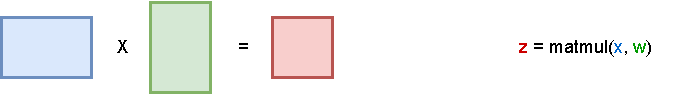
\includegraphics[width=.9\textwidth]{single_card.pdf}
    \end{frame}


    \begin{frame}
        \frametitle{Tensor Sharding}

        \centering
        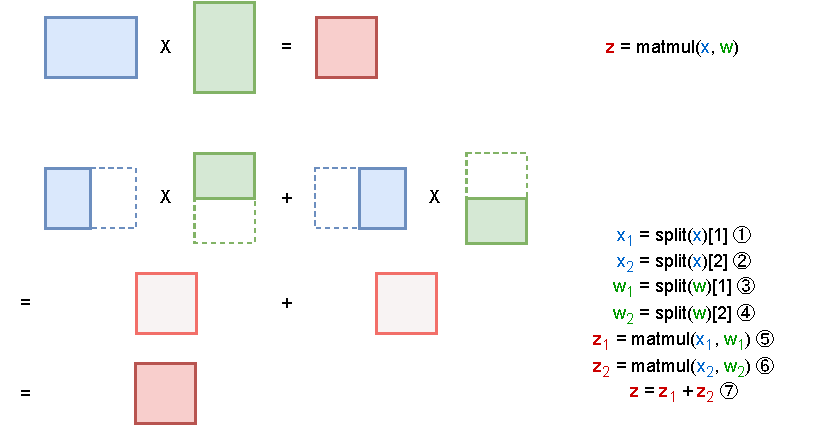
\includegraphics[width=.85\textwidth]{transformation.pdf}
    \end{frame}


    \begin{frame}
        \frametitle{SPMD Parallelism}

        \centering
        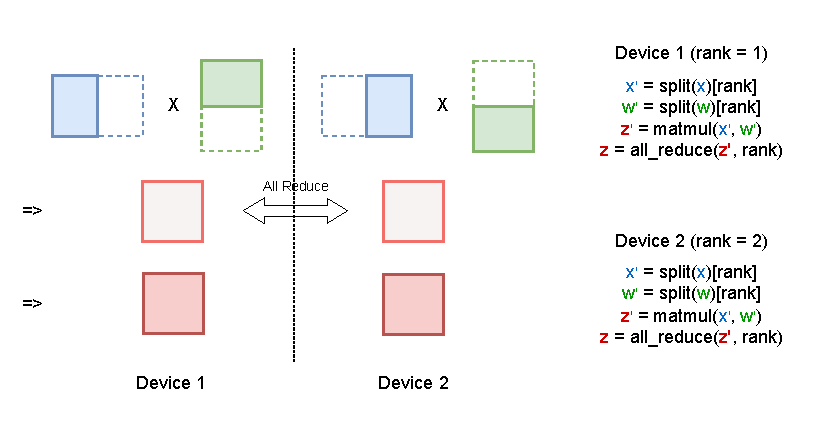
\includegraphics[width=.85\textwidth]{spmd.pdf}
    \end{frame}

    \begin{frame}
        \frametitle{Multiple Ways to Parallelize a Tensor Program}

        \centering
        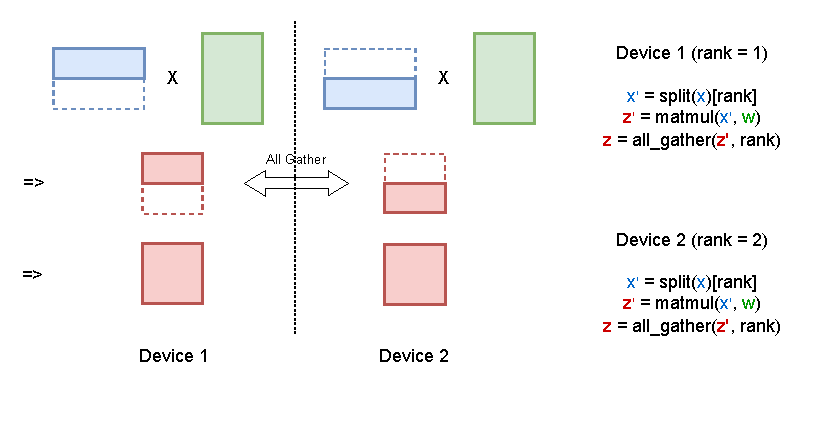
\includegraphics[width=.85\textwidth]{spmd2.pdf}
    \end{frame}

    \begin{frame}
        \frametitle{SPMD Parallelism on Heterogeneous Clusters}

        \centering
        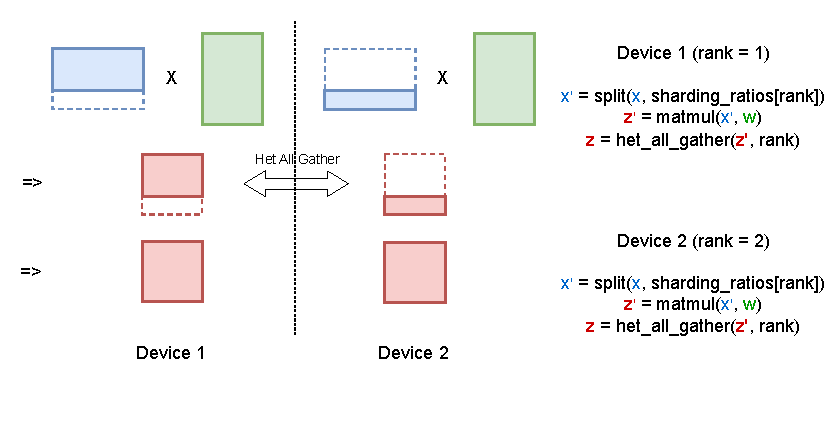
\includegraphics[width=.85\textwidth]{hetspmd.pdf}
    \end{frame}

    \begin{frame}
        \frametitle{Challenges}

        \begin{center}
            \vspace{-3em}
            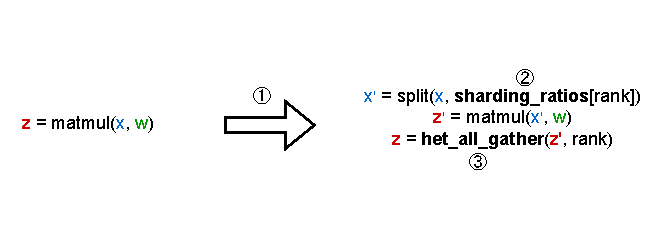
\includegraphics[width=.85\textwidth]{goal.pdf}
        \end{center}
        \vskip -2em

        \circled{1} How to generate a distributed program that produces equivalent results \\
        \circled{2} How to determine the sharding ratios for the heterogeneous devices \\
        \circled{3} How to choose the communication method on heterogeneous networks
    \end{frame}



    \begin{frame}
        \centering
        \begin{beamercolorbox}[sep=8pt,center,shadow=true,rounded=true]{title}
          \usebeamerfont{title}Automated Program Synthesis\par%
        \end{beamercolorbox}
    \end{frame}

    \begin{frame}
        \frametitle{Automated Program Synthesis}

        \begin{columns}
            \begin{column}{0.46\textwidth}
                We synthesize a distributed program from scratch on a distributed instruction set that emulates the single-device program.
                \vskip 1em
                To ensure the equivalence of the original and synthesized programs, we formalize the semantics of the single-device program and generate the distributed program under a semantic constraint.
            \end{column}
            \begin{column}{0.54\textwidth}
                \centering
                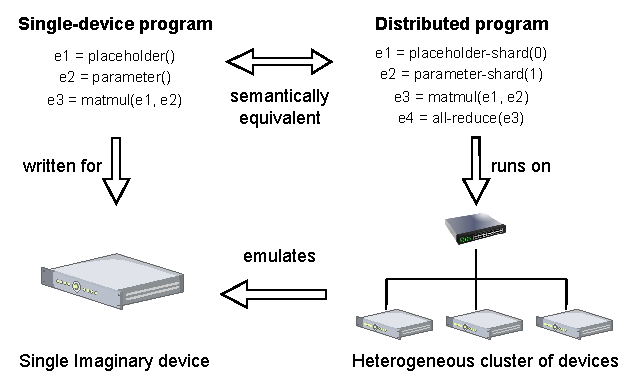
\includegraphics[width=\textwidth]{emulator.pdf}
            \end{column}
        \end{columns}
    \end{frame}

    \begin{frame}
        \frametitle{Automated Program Synthesis}

        \begin{columns}
            \begin{column}{0.46\textwidth}
                \centering
                \includegraphics[page=7,trim=56.82bp 616.43bp 324.91bp 69.14bp,clip,scale=.85]{paper.pdf}
                \vskip .5em
                Syntax Rules
            \end{column}
            \begin{column}{0.54\textwidth}
                \centering
                \includegraphics[page=8,trim=51.72bp 545.40bp 309.34bp 72.99bp,clip,scale=.9]{paper.pdf}
                \vskip .5em
                Semantic Rules
            \end{column}
        \end{columns}
    \end{frame}



    \begin{frame}
        \frametitle{Load Balancing}

        \begin{center}
            \vspace{-3em}
            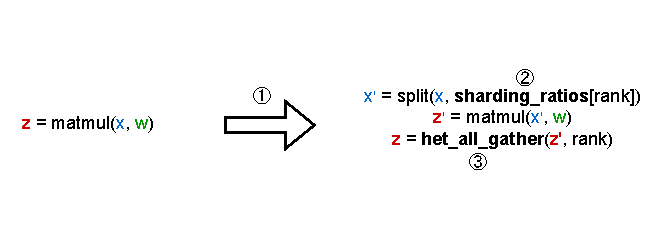
\includegraphics[width=.85\textwidth]{goal.pdf}
        \end{center}
        \vskip -2em

        \circled{1} How to generate a distributed program that produces equivalent results \\
        \textbf{\circled{2} How to determine the sharding ratios for the heterogeneous devices} \\
        \circled{3} How to choose the communication method on heterogeneous networks
    \end{frame}

    \begin{frame}
        \frametitle{Cost Model}

        As synchronization among devices is required during collective communication, the execution of the distributed program can be divided into stages.

        \vskip 2em
        \centering
        \includegraphics[page=6,trim=64.08bp 633.23bp 332.38bp 67.73bp,clip,scale=1.1]{paper.pdf}
    \end{frame}

    \begin{frame}
        \frametitle{Optimization Problem Formulation}

        \begin{center}
            \vspace{-1em}
            \includegraphics[page=10,trim=335.25bp 397.28bp 71.11bp 321.51bp,clip]{paper.pdf}
        \end{center}

        \textbf{Q}: distributed program \\
        \textbf{B}: sharding ratios for the devices \\
        \textbf{comm}, \textbf{comp}: linear models of communication and computation times.
    \end{frame}

    \begin{frame}
        \frametitle{Communication Optimization}

        \begin{center}
            \vspace{-3em}
            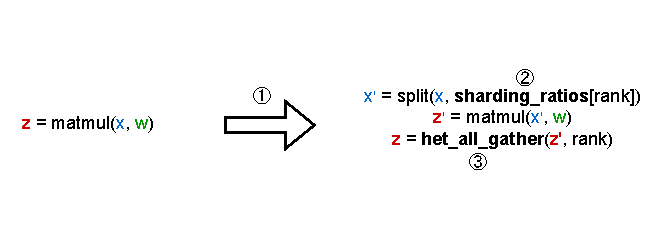
\includegraphics[width=.85\textwidth]{goal.pdf}
        \end{center}
        \vskip -2em

        \circled{1} How to generate a distributed program that produces equivalent results \\
        \circled{2} How to determine the sharding ratios for the heterogeneous devices \\
        \textbf{\circled{3} How to choose the communication method on heterogeneous networks}
    \end{frame}

    \begin{frame}
        \frametitle{Optimal Communication Method Depends}

    \end{frame}

    \begin{frame}
        \frametitle{Sufficient Factor Broadcasting}

    \end{frame}



    \begin{frame}
        \centering
        \begin{beamercolorbox}[sep=8pt,center,shadow=true,rounded=true]{title}
          \usebeamerfont{title}Implementation\par%
        \end{beamercolorbox}
    \end{frame}

    \begin{frame}
        \frametitle{Implementation}

        \begin{columns}
            \begin{column}{0.5\textwidth}
                We implement HAP on top of PyTorch.
                \vskip 1em
                We round the sharding ratios to ensure that the program runs with any number of devices, even if it does not evenly divide the tensor dimensions.
            \end{column}
            \begin{column}{0.5\textwidth}
                \centering
                \includegraphics[page=11,trim=342.71bp 491.17bp 83.58bp 69.93bp,clip,scale=.9]{paper.pdf}
            \end{column}
        \end{columns}
    \end{frame}

    \begin{frame}
        \frametitle{Implementation}

        \begin{itemize}
            \setlength{\itemsep}{.8em}
            \item \textbf{Annotator}: Label the possible sharding methods for each operator, infer the tensor sizes, and estimate the FLOPs.
            \item \textbf{Strategy Searcher}: Take annotated graph as input and search for the optimal sharding strategy.
            \item \textbf{Compiler}: Modify the graph according to the strategy and applies Duplex.
        \end{itemize}

        \note{The annotator encodes the domain knowledge, the other two components are generic. To add support for a new operator, only the annotator needs to be modified.}
    \end{frame}

    \begin{frame}
        \centering
        \begin{beamercolorbox}[sep=8pt,center,shadow=true,rounded=true]{title}
          \usebeamerfont{title}Evaluation\par%
        \end{beamercolorbox}
    \end{frame}

    \begin{frame}
        \frametitle{Experimental Setup}

        \begin{itemize}
            \setlength{\itemsep}{.8em}
            \item \textbf{Testbed}: 8 machines on public cloud, each with 8 V100 GPUs and NVLink, connected by 10Gbps network.
            \item \textbf{Benchmarks}: BERT (language modeling) and ViT (image classification), with two variants of MoE layers, SGMoE and Switch.
            \item \textbf{Baselines}: DeepSpeed, FastMoE, PyTorch DDP, and Horovod.
        \end{itemize}
    \end{frame}

    \begin{frame}
        \frametitle{Per-iteration training time}

        \includegraphics[page=10,trim=2.2cm 20.5cm 2.2cm 2.6cm,clip,scale=0.8]{paper.pdf}

        \vskip 1em
        HiDup outperforms baselines when scaling up, because the collective communication becomes slower with more cards
        and HiDup can mitigate the increased communication overhead with our Duplex design.
    \end{frame}

    \begin{frame}
        \frametitle{Single Machine Performance}

        \includegraphics[page=10,trim=2.2cm 15cm 2.2cm 8.1cm,clip,scale=0.8]{paper.pdf}

        \vskip .5em
        Pure-DP methods perform well with high bandwidth. HiDup automatically identifies similar strategies and achieves
        comparable performance despite of the additional overheads introduced by our Duplex design.
    \end{frame}

    \begin{frame}
        \frametitle{Per-iteraion time breakdown}

        \includegraphics[page=13,trim=2.2cm 21cm 2.2cm 3.5cm,clip,scale=0.81]{paper.pdf}

        HiDup's total time is similar to the baselines, but it achieves shorter wall time by overlapping computation
        and communication.
    \end{frame}

    \begin{frame}
        \frametitle{SPMD Strategy}

        \begin{columns}
            \begin{column}{0.48\textwidth}
                HiDup generates different strategies for the same model on different clusters.

                \vskip 1em
                It automatically identifies expert-designed strategies for common models.
            \end{column}
            \begin{column}{0.55\textwidth}
                \centering
                \vskip -2em
                \includegraphics[page=13,trim=2cm 12.9cm 11.2cm 6.8cm,clip,scale=0.84]{paper.pdf}
            \end{column}
        \end{columns}
    \end{frame}


    \appendix

    \begin{frame}
        \vskip 1em

        \vskip 1em
        \centering
        {\huge Thank you!}
        \vskip 1em
        Email: swzhang\,@\,cs.hku.hk

    \end{frame}
\end{document}
